\documentclass[tikz,border=8pt]{standalone}
% Shared look for every TikZ diagram. Load with % Shared look for every TikZ diagram. Load with % Shared look for every TikZ diagram. Load with \input{../../tools/tikz-style.tex}
\usepackage[T1]{fontenc}
\usepackage{lmodern}
\renewcommand{\sfdefault}{lmr}  % diagrams use the same serif as the text
\usetikzlibrary{arrows.meta, positioning, shapes.geometric, calc, fit, backgrounds}
\definecolor{cblue}{HTML}{4C78A8}
\definecolor{corange}{HTML}{F58518}
\definecolor{cgreen}{HTML}{54A24B}
\definecolor{cred}{HTML}{E45756}
\definecolor{cpurple}{HTML}{B279A2}
\definecolor{cgrey}{HTML}{6B6B6B}
\tikzset{
  every picture/.style={font=\sffamily, line width=1.2pt},
  box/.style={draw=#1, fill=#1!12, rounded corners=4pt, align=center, inner sep=7pt, minimum height=1.1cm},
  box/.default=cgrey,
  arrow/.style={-{Stealth[length=3mm]}, draw=cgrey, line width=1.4pt},
  title/.style={font=\sffamily\bfseries\Large},
  note/.style={font=\sffamily\small, text=cgrey, align=center},
}
\AtBeginDocument{\hyphenpenalty=10000 \exhyphenpenalty=10000}

\usepackage[T1]{fontenc}
\usepackage{lmodern}
\renewcommand{\sfdefault}{lmr}  % diagrams use the same serif as the text
\usetikzlibrary{arrows.meta, positioning, shapes.geometric, calc, fit, backgrounds}
\definecolor{cblue}{HTML}{4C78A8}
\definecolor{corange}{HTML}{F58518}
\definecolor{cgreen}{HTML}{54A24B}
\definecolor{cred}{HTML}{E45756}
\definecolor{cpurple}{HTML}{B279A2}
\definecolor{cgrey}{HTML}{6B6B6B}
\tikzset{
  every picture/.style={font=\sffamily, line width=1.2pt},
  box/.style={draw=#1, fill=#1!12, rounded corners=4pt, align=center, inner sep=7pt, minimum height=1.1cm},
  box/.default=cgrey,
  arrow/.style={-{Stealth[length=3mm]}, draw=cgrey, line width=1.4pt},
  title/.style={font=\sffamily\bfseries\Large},
  note/.style={font=\sffamily\small, text=cgrey, align=center},
}
\AtBeginDocument{\hyphenpenalty=10000 \exhyphenpenalty=10000}

\usepackage[T1]{fontenc}
\usepackage{lmodern}
\renewcommand{\sfdefault}{lmr}  % diagrams use the same serif as the text
\usetikzlibrary{arrows.meta, positioning, shapes.geometric, calc, fit, backgrounds}
\definecolor{cblue}{HTML}{4C78A8}
\definecolor{corange}{HTML}{F58518}
\definecolor{cgreen}{HTML}{54A24B}
\definecolor{cred}{HTML}{E45756}
\definecolor{cpurple}{HTML}{B279A2}
\definecolor{cgrey}{HTML}{6B6B6B}
\tikzset{
  every picture/.style={font=\sffamily, line width=1.2pt},
  box/.style={draw=#1, fill=#1!12, rounded corners=4pt, align=center, inner sep=7pt, minimum height=1.1cm},
  box/.default=cgrey,
  arrow/.style={-{Stealth[length=3mm]}, draw=cgrey, line width=1.4pt},
  title/.style={font=\sffamily\bfseries\Large},
  note/.style={font=\sffamily\small, text=cgrey, align=center},
}
\AtBeginDocument{\hyphenpenalty=10000 \exhyphenpenalty=10000}

\begin{document}
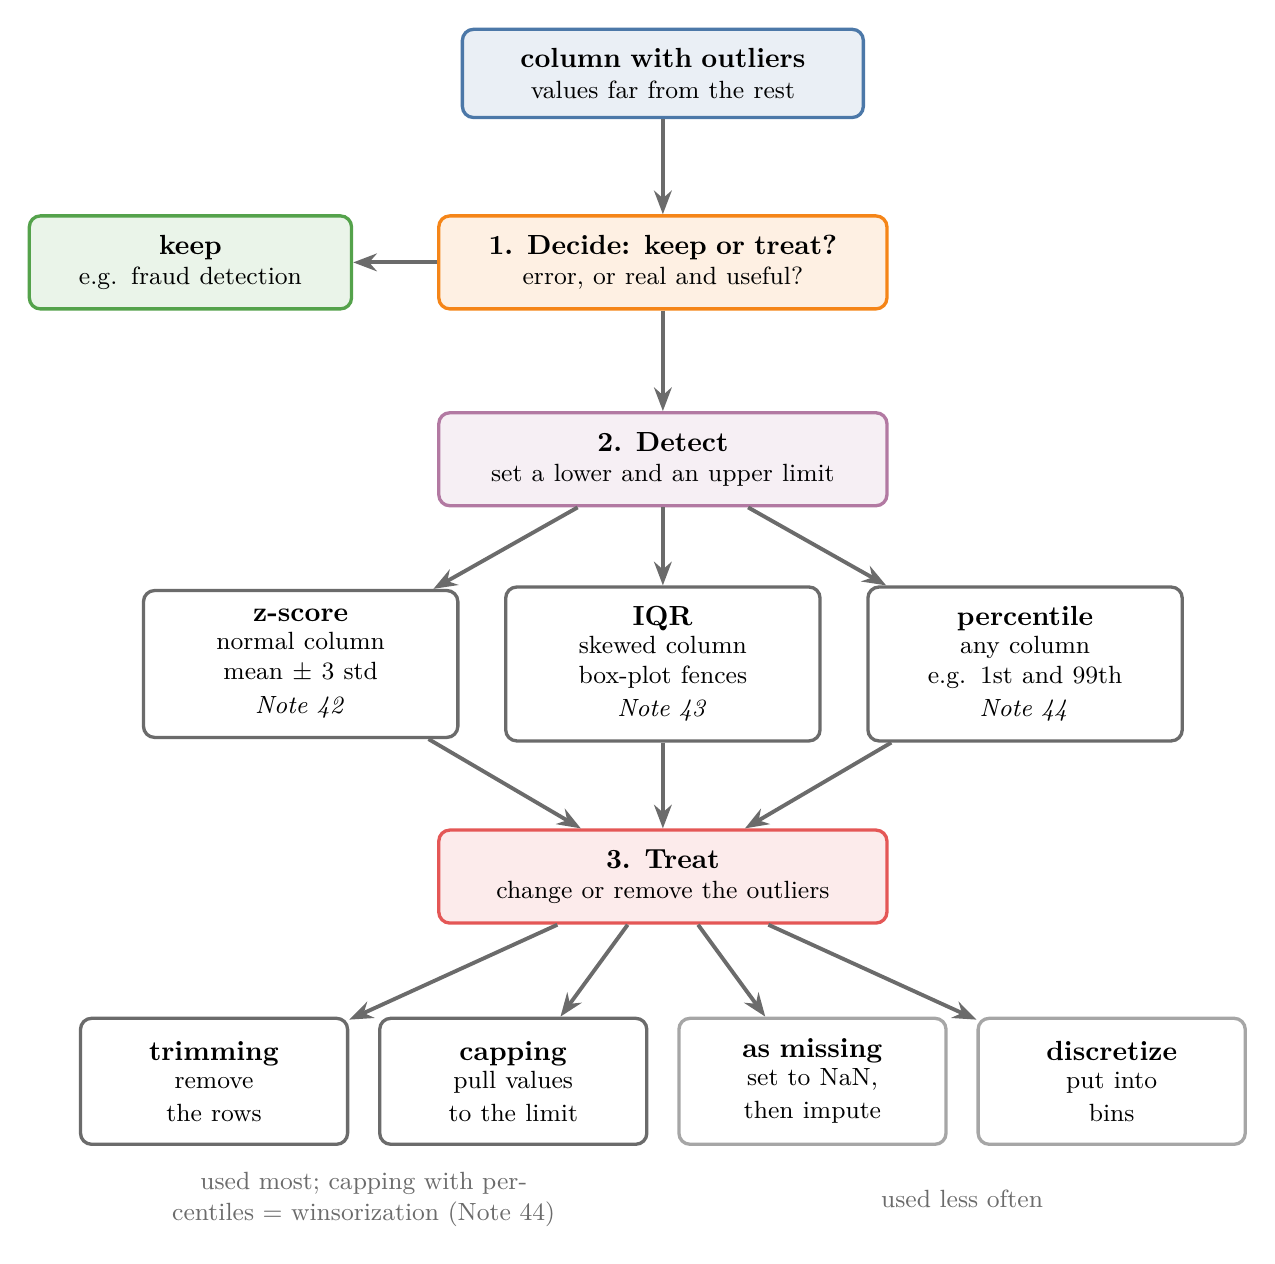
\begin{tikzpicture}
  \node[box=cblue, text width=4.6cm] (in) at (0,0) {\textbf{column with outliers}\\[-1pt]\small values far from the rest};
  % decision
  \node[box=corange, text width=5.2cm] (dec) at (0,-2.4) {\textbf{1. Decide: keep or treat?}\\[-1pt]\small error, or real and useful?};
  \draw[arrow] (in) -- (dec);
  \node[box=cgreen, text width=3.6cm] (keep) at (-6,-2.4) {\textbf{keep}\\[-1pt]\small e.g. fraud detection};
  \draw[arrow] (dec) -- (keep);
  % detect
  \node[box=cpurple, text width=5.2cm] (det) at (0,-4.9) {\textbf{2. Detect}\\[-1pt]\small set a lower and an upper limit};
  \draw[arrow] (dec) -- (det);
  \node[box=cgrey, fill=white, text width=3.5cm] (z) at (-4.6,-7.5) {\textbf{z-score}\\[-1pt]\small normal column\\ mean $\pm$ 3 std\\ \textit{Note 42}};
  \node[box=cgrey, fill=white, text width=3.5cm] (iqr) at (0,-7.5) {\textbf{IQR}\\[-1pt]\small skewed column\\ box-plot fences\\ \textit{Note 43}};
  \node[box=cgrey, fill=white, text width=3.5cm] (pct) at (4.6,-7.5) {\textbf{percentile}\\[-1pt]\small any column\\ e.g. 1st and 99th\\ \textit{Note 44}};
  \draw[arrow] (det) -- (z); \draw[arrow] (det) -- (iqr); \draw[arrow] (det) -- (pct);
  % treat
  \node[box=cred, text width=5.2cm] (tr) at (0,-10.2) {\textbf{3. Treat}\\[-1pt]\small change or remove the outliers};
  \draw[arrow] (iqr) -- (tr);
  \draw[arrow] (z) -- (tr); \draw[arrow] (pct) -- (tr);
  \node[box=cgrey, fill=white, text width=2.9cm, minimum height=1.6cm] (trim) at (-5.7,-12.8) {\textbf{trimming}\\[-1pt]\small remove\\ the rows};
  \node[box=cgrey, fill=white, text width=2.9cm, minimum height=1.6cm] (cap) at (-1.9,-12.8) {\textbf{capping}\\[-1pt]\small pull values\\ to the limit};
  \node[box=cgrey, fill=white, text width=2.9cm, minimum height=1.6cm, draw=cgrey!60] (miss) at (1.9,-12.8) {\textbf{as missing}\\[-1pt]\small set to NaN,\\ then impute};
  \node[box=cgrey, fill=white, text width=2.9cm, minimum height=1.6cm, draw=cgrey!60] (bin) at (5.7,-12.8) {\textbf{discretize}\\[-1pt]\small put into\\ bins};
  \draw[arrow] (tr) -- (trim); \draw[arrow] (tr) -- (cap); \draw[arrow] (tr) -- (miss); \draw[arrow] (tr) -- (bin);
  \node[note, text width=6.4cm] at (-3.8,-14.3) {used most; capping with percentiles = winsorization (Note 44)};
  \node[note, text width=6.4cm] at (3.8,-14.3) {used less often};
\end{tikzpicture}
\end{document}
